\documentclass[tikz, border=5mm]{standalone}
\usepackage{textcomp}
\usetikzlibrary{arrows.meta,decorations.markings,fit,calc, positioning}

\definecolor{componentColor}{RGB}{210,210,210}
\definecolor{systemColor}{RGB}{230,230,230}

\tikzset{component/.append style={fill=componentColor, align=center, draw, minimum width=2cm, minimum height=1.5cm, rounded corners=.3cm}}
\tikzset{system/.style={component, fill=systemColor, rounded corners=0cm}}


\begin{document}

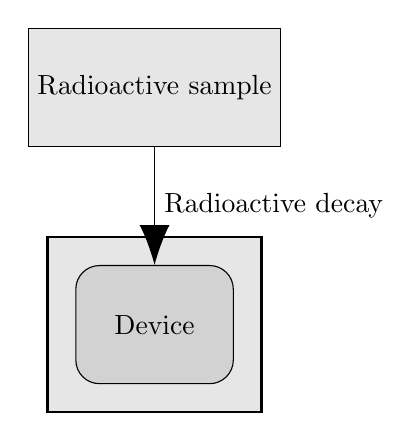
\begin{tikzpicture}[node distance=1.5cm and 3cm]
% Nodes
\pgfdeclarelayer{background}
\pgfsetlayers{background,main}

\node (chamber) [component] {Device};
\node (sample) [system, above=of chamber] {Radioactive sample};


\begin{pgfonlayer}{background}
\node[system, draw, thick, inner xsep=1em, inner ysep=1em, fit= (chamber) ] {};
\end{pgfonlayer}

% Connectors
\begin{scope}[->]

\draw [-{Latex[scale=3.0]}] (sample) -- node[anchor=west, minimum width=.25cm, draw=none] {Radioactive decay} (chamber);

\end{scope}

\end{tikzpicture}
\end{document}
